\providecommand{\main}{../../main}
\documentclass[../../main.tex]{subfiles}


\begin{document}

\chapter{Neural Networks based conditions in Phase-2 Global Trigger}
\chaptermark{Neural Networks at GT}
\label{sec:P2GT}

Phase-2 Global Trigger has the ambition to implement neural network based conditions alongside the usual algorithms already in use in Run-3, such as cut on a specific or combination of reconstructed particle properties. These neural network based conditions must meet some stringent requirements in order to be implemented in the global trigger algorithm chain.  
\begin{itemize}
    \item \textbf{Latency}: The upgrade foresees for the whole GT a total latency of $1\mu s$ corresponding to 40 BXs, running neural network inference requires time of the order of hundreds of nanoseconds to microseconds if not optimized accordingly.
    \item \textbf{Resources}: In general neural networks are resource hungry, heavy optimization must take place during and after training in order to to be implemented alongside the  $\sim1000$ cut-based algorithms.  
\end{itemize}

In the following sections the VHDL code produces to integrate a simple neural network bin the Phase-2 Global Trigger is shown, in particular the steps needed to translate a Keras model into pure VHDL code are highlighted, taking into account also data conditioning and the various interfaces required.

\section{Global Trigger Algorithm board}
\label{sec:Gt-algo-board}

\begin{figure}[h]
    \centering
    \includegraphics[width=0.90\textwidth]{sections/05/Images/GT-algo.png}
    \caption{Phase-2 prototype firmware.}
    \label{fig:P2GT}
\end{figure}  

In Fig. \ref{fig:P2GT} the Global Trigger firmware is depicted, highlighting the simplified signal data path from the detectors up to the Data AQuisition (DAQ) systems. Following the data coming from the various subsystems to the algorithm board, these submodules are found:
\begin{itemize}
    \item De-multiplexers: Reconstructed particle signals arrive in a time multiplexed fashion, they need to be packed in collections ready to be analysed by the algorithms;
    \item Reformatting data to meet the GT common format and SLR distribution\footnote{The target board is the Virtex Ultrascale+ VU13P made of 4 SLRs};
    \item Algorithm module made of cut-based conditions and neural network based ones:
    \item HLT objects bits: bits that contain information on objects contribution to a firing algorithm and other useful information to sent to the high level trigger subsystem;
    \item Algorithm combinatorial logic between algorithm results.
\end{itemize}
The algorithm results are sent to the Final-OR board ready to be pre-scaled and monitored, the final step is to evaluate the logic OR of such results and forward it to the TCDS-2, the details of the Final-Or board can be found in Chapter \ref{sec:Finor}.



In the following sections a simple neural network topological trigger will be taken as example to present the necessary steps for the integration in the Phase-2 Global Trigger firmware. 
    
\section{Topological trigger}
\sectionmark{Topological trigger}
\label{sec:P2GT_NN}

In this section the target neural network is described, highlighting the main advantages over the generic cut-based algorithms and the related drawbacks of such implementation. The base model was developed in a previous work\cite{Ihor_thesis} by the Hamburg Trigger Menu group.  

The module has the aim to discriminate a particular signal event from the background, minimizing the false negative rate and false positive rate. False negative rate means that a signal event has been labeled as background and is consequently rejected, this is a data loss in fact once is rejected an event it cannot be restored. The false positive rate plays a role in the final trigger rate of such conditions, the maximum total trigger rate is a fixed number determined by hardware limitations, in the case of Phase-2 this number is 750kHz, reducing the false positive rate will improve the overall signal efficiency.     


\subsection{Data sets}
\label{sec:NN-dataset}
Here the samples of signal processes and the background process studied in this thesis are presented and the key differences between these processes is discussed, which
play a crucial role for the development of trigger selection algorithms. The target system will be the Phase-2 Global Trigger and since no real datasets are available, all presented datasets come from a Monte Carlo simulation employing Pythia8 [32]. Data set distributions are shown in appendix \ref{sec:App_Model}.

Two processes are considered:
\begin{itemize}
    \item \textbf{$HH \xrightarrow{} b \Bar{b}WW$}: Main process to study, in this work only di-Higgs decay with one lepton in the final state is considered, in particular the electron and the muon channel.
    \item \textbf{$t\Bar{t} \xrightarrow{} b \Bar{b}WW$}: Process with the same final state as the di-Higgs decay, it has a harder $p_T$ spectrum.
    \item \textbf{MinBias}: as background signal is taken the \textit{minimum bias} events, they include inelastic scattering processes occurring in $p-p$ collisions with a minimum momentum transfer. 
\end{itemize}

The Fig. \ref{fig:fayman} presents Feynman diagrams for such processes.

%\begin{figure*}[ht] 
%  \begin{minipage}[b]{0.5\linewidth}
%    \centering
%    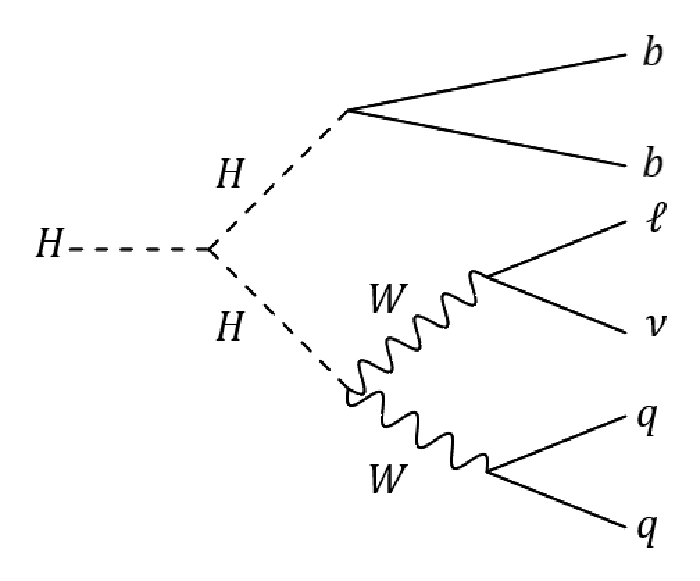
\includegraphics[width=.75\linewidth]{sections/05/Images/hh.pdf}
%    
%    \caption*{$HH \xrightarrow{} b \Bar{b}WW$ process} 
%    \vspace{4ex}
%  \end{minipage}%%
%  \begin{minipage}[b]{0.5\linewidth}
%    \centering
%    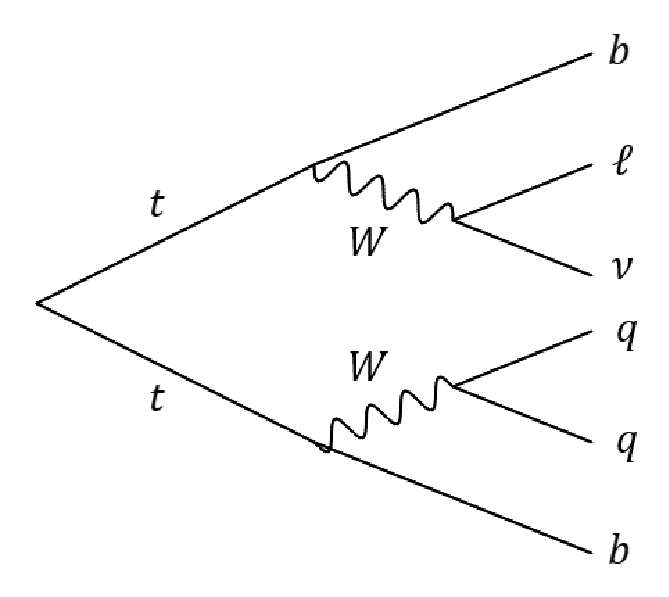
\includegraphics[width=.75\linewidth]{sections/05/Images/ttbar.pdf} 
%    \caption*{$ t \Bar{t} \xrightarrow{} b \Bar{b}WW$ process} 
%    \vspace{4ex}
%  \end{minipage} 
%  \caption{Feynman diagrams of the studied processes} 
%  \label{fig:fayman}
%\end{figure*}


\begin{figure}[htp]
    \begin{minipage}{0.5\linewidth}
        \centering
        \subfloat[$HH \xrightarrow{} b \Bar{b}WW$ process]{
            \adjustbox{valign=c}{%
                \includestandalone[mode=tex, height=6cm]{sections/05/hhww}
            }%
            % \vphantom{\includestandalone[mode=tex, width=\textwidth]{\figpath/VBFToH}}
        }
    \end{minipage}%
    \begin{minipage}{0.5\linewidth}
        \centering
        \subfloat[$ t \Bar{t} \xrightarrow{} b \Bar{b}WW$ process]{
            \adjustbox{valign=c}{%
                \includestandalone[mode=tex, height=6cm]{sections/05/ttbar}
            }%
        }
    \end{minipage}%
    
    \caption{Feynman diagrams of the studied processes}
    \label{fig:fayman}
    
\end{figure}


Table \ref{tab:cross_sec_table} shows the cross sections of the studied processes at $\sqrt{s} = 13 TeV$. For the $HH$ and $t\Bar {t}$ processes these are the theoretical estimations. The minimum bias cross section is measured by the CMS detector. The Higgs Boson pair production has four orders of magnitude lower cross section than the $t\Bar {t}$ process.

\begin{center}
    \begin{table}[h]
    \centering
    \begin{tabular}{|c|c|c|c|}
        \hline
        Process & $\sigma[fb]$ & Uncertainty[PDF+$\alpha S$] & Available samples \\
        \hline
        $HH$         & 31.05 & $\pm 3.0 \%$ & $19\times10^3$ \\
        $t\Bar {t}$  & $833.9\times 10^{3}$ & $\pm 2.5 \%$ & $298\times10^3$ \\
        MinBias & $67.5\times 10^{12}$ & $\pm 1.18 \%$(syst) $\pm 2.37 \%$(lumi) & $761\times10^3$ \\
        \hline
    \end{tabular}
    \caption{Processes cross section at $\sqrt{s}=13TeV$}
    \label{tab:cross_sec_table}
    \end{table}
\end{center}

\subsection{Neural Network architecture}
\label{P2GT_NN}
The selection algorithm has to distinguish between the processes that are of interest and the minimum bias. Thus, the goal of the developed neural network is the classification of the incoming events. The output of a such neural network is a score that quantifies how near the signal is to a target one, then a threshold is set and if the score is above this values the trigger fires and the signal is stored. 

Table \ref{tab:Input_obj} presents the L1 trigger objects that were used for this study.
All these objects are inputs of the Global Trigger. Since all studied processes are Monte Carlo simulations the generator level information is available. The information about each type of process will be available during the training of the neural network.

\begin{center}
    \begin{table}[h]
    \centering
    \begin{tabular}{|c|c|c|c|c|}
        \hline
        L1T Objects & Subsystem &\multicolumn{3}{c|}{Variables} \\
        \hline
        First 4 jets        & CL2 & $p_T$ & $\eta$   & \cellcolor{gray!25}$\phi$ \\
        First 2 electrons   & CL2 & $p_T$ & $\eta$   & \cellcolor{gray!25}$\phi$ \\
        First 2 muons       & GMT & $p_T$ & $\eta$   & \cellcolor{gray!25}$\phi$ \\
        Missing energy      & CL2 & $E_T^{miss}$ & - & \cellcolor{gray!25}$\phi$ \\
        \hline
    \end{tabular}
    \caption{Input objects of the studied neural network}
    \label{tab:Input_obj}
    \end{table}
\end{center}

In this section binary classifiers are considered, their name derives form the task that they are required to accomplish, in fact a classification between signal and background of the input. Here two different binary classifiers are studied, one for each of the two lepton channels. Firstly a baseline model is evaluated with \textit{Keras}, then a quantized version is produced and finally the hardware implementation is evaluated.  
Multiple scores are given to each model to judge the best one, in particular the scores are:
\begin{itemize}
    \item \textbf{Accuracy}: Percentage of correct labels predicted, in a trigger environment this parameter is not useful\footnote{In this particular case the background data set is larger than the signal one, the neural network can achieve high accuracy giving background label at every incoming signal}, nevertheless it gives some information on the goodness of the model, the threshold of the sigmoid output is set to 0.5 .
    \item \textbf{AUC}: Area Under ROC Curve explained in section \ref{sec:roc}, it quantifies how good the model is with respect to the false positive and true positive rates.
    \item \textbf{Signal$_{Eff}$}: This evaluate the signal efficiency, for the neural network model it is evaluated at 10$kHz$ MinBias rate.
\end{itemize} 
Such scores are evaluated with the full test data set described below.
Baseline models are trained with the $t \Bar{t}$ dataset and a background factor of 10, which means that in the final data sample for every event signal 10 background signals are present. The dataset is split in training and validation set with 0.75 and 0.25 fractions respectively. As test set the $HH$ sample with a background factor of 191\footnote{It was used the whole MinBias dataset made of $761\times10^3$ samples} was used.  

The training parameters are summarized below:
\begin{itemize}
    \item Keras framework
    \item 30 epochs
    \item ADAM optimizer
    \item Binary cross-entropy loss function
    \item No pruning applied
    \item Single precision weights and biases
\end{itemize}

In the figures \ref{fig:baseline_models} ROC curves for the two lepton channel models are shown, as a comparison the signal efficiency of the respective Single Lepton trigger with $p_T$ threshold set at 30 $GeV$ for electrons and 20 $GeV$ for muons\cite{L1T-2up} is given.  

\begin{figure*}[ht] 
  \label{ fig7} 
  \begin{minipage}[b]{0.5\linewidth}
    \centering
    \includegraphics[width=.95\linewidth]{sections/05/Images/baseline_1ele_ROC.png} 
    %\caption{Electron channel} 
    \vspace{4ex}
  \end{minipage}%%
  \begin{minipage}[b]{0.5\linewidth}
    \centering
    \includegraphics[width=.95\linewidth]{sections/05/Images/baseline_1mu_ROC.png} 
    %\caption{Muon channel} 
    \vspace{4ex}
  \end{minipage} 
  \caption{Electron channel in the left and muon channel in the right. Single Lepton triggers performance are show with $p_T$ threshold set at 30 and 20 $GeV$ respectively.}
  \label{fig:baseline_models}
\end{figure*}

The baseline model features are summarized in the table \ref{tab:baseline_NN}. The two baseline models feature the same architecture made up of three hidden layers, with 64, 32 and 32 nodes respectively. The cut-based algorithm performs worse than the neural networks models whit lower AUC and signal efficiency.

\begin{center}
    \begin{table}[h]
    \centering
    \begin{tabular}{|c|c|c|c|c|c|c|c|}
        \hline
        \multirow{2}{*}{Label} & \multirow{2}{*}{Arch} & \multicolumn{2}{c|}{Activation} & \multirow{2}{*}{Accuracy} & \multirow{2}{*}{AUC} & \multirow{2}{*}{Sig$_{eff}$[\%]} & \multirow{2}{*}{Rate[kHz]} \\
        \cline{3-4}
        && Hidden & Output& [\%] &&&\\
        \hline
        Baseline $e$ & 64/32/32 & ReLU & Sigmoid & 99.6 & 0.995 & 64.9 & 10 \\
        Single Electron & $p_T>30GeV$ & - & - & 99.5 & 0.720 & 50.6 & 51 \\
        %Double Jets & $p_T^{0-1} \geq 95,95GeV$ & - & - & 99.6 & 0.725 & 45.2 & 37 \\
        Baseline $\mu$ & 64/32/32 & ReLU & Sigmoid & 99.8 & 0.995 & 79.1 & 10 \\
        Single Muon & $p_T>20GeV$ & - & - & 99.7 & 0.762 & 52.4 & 8  \\
        %Double Jets & $p_T^{0-1} \geq 95,95GeV$ & - & - & 99.6 & 0.713 & 42.8 & 37 \\
        \hline
    \end{tabular}
    \caption{Baseline models and Single Lepton triggers characteristics.}
    \label{tab:baseline_NN}
    \end{table}
\end{center}

Single Lepton Trigger is part of the so-called cut-based conditions, in fact a threshold and a condition are set and everything that does not satisfy such cut is rejected. In this particular case all signal with a $p_T$ greater or equal to the threshold will assert the algorithm. This type of triggers are the simplest ones, but they offer worse performance than algorithms with more advanced computations; usually they are combined together to get a specific signal signature.

\section{Hardware Implementation}
\label{sec:P2GT_Imp}

Once the baseline model has been trained the next step will be to optimize it to meet the aforementioned requirements for the hardware implementation, in the next sections it will be shown how to obtain a significant resource reduction without significantly compromising the performance of the model. 
Firstly the inputs that do not contribute to signal-background distinction have been taken out of the data set, such signal are in fact the $\phi$ component of the reconstructed particle. A simple optimization can be done on the input variables, in fact all the signal are supposed to be isotropic. This results a total of 17 features out of the 26 available.   

Currently the GT firmware supports three different clock frequencies: 40MHz, 240MHz and 480MHz. 480MHz has been chosen to match the other algorithms\footnote{480MHz was chosen to lower double object conditions latency} already implemented, the neural network on the other hand can support 240MHz or 480MHz. A study on these frequencies can be found in section \ref{sec:P2GT_clock test}.
    
\subsection{Quantization}
\label{sec:P2GT_Comp}

\begin{figure*}[h] 
  \label{ fig7} 
  \begin{minipage}[b]{0.5\linewidth}
    \centering
    \includegraphics[width=.95\linewidth]{sections/05/Images/Quant_AUC_1ele.png} 
    \vspace{4ex}
  \end{minipage}%%
  \begin{minipage}[b]{0.5\linewidth}
    \centering
    \includegraphics[width=.95\linewidth]{sections/05/Images/Quant_SigEff_1ele.png}
    \vspace{4ex}
  \end{minipage}
  \caption{Performance degradation with respect to different weights and biases bit width.} 
  \label{fig:quantization_plots}
\end{figure*}

As it was mentioned in section \ref{sec:FPGA_elements} the silicon dedicated to arithmetic operations is limited in number and bit-width of the factors\footnote{depending on the FPGA generation it varies from 25x18 bits for the 7-series up to 27x18 for the Ultrascale+}.  
In this particular case the multiplication is done between input value and the weight, which means that they are capped at 27 and 18 bits respectively, beyond that more DSPs and LUTs will be used.   

In this and next tests a simple 2-hidden layer model is considered. Two quantizations will be performed:
\begin{itemize}
    \item Quantization Aware Training \textbf{\acrshort{qat}}: The training algorithm is aware of the weight quantization leading to a more aggressive bit width reduction. Python library \textit{QKeras}\cite{qkeras}\footnote{As its name suggests this library is just a variation of the Tensorflow Keras frame work, it offers quantized version of the most used layers and activation functions} is used to do so.
    \item Post Training Quantization \textbf{\acrshort{pqt}}: After the training step the inputs bit-width is tuned to preserve as much as possible the NN performances. It is possible to quantize further weights and biases, but they are generally heavily optimized by the QAT step, so only input precision is generally studied.
\end{itemize}


\begin{figure*}[h] 
  \label{ fig7} 
  \begin{minipage}[b]{0.5\linewidth}
    \centering
    \includegraphics[width=.9\linewidth]{sections/05/Images/Quant_LUT_1ele.png} 
    \vspace{2ex}
  \end{minipage}%%
  \begin{minipage}[b]{0.5\linewidth}
    \centering
    \includegraphics[width=.9\linewidth]{sections/05/Images/Quant_FF_1ele.png}
    \vspace{2ex}
  \end{minipage} 
  \begin{minipage}[b]{0.5\linewidth}
    \centering
    \includegraphics[width=.9\linewidth]{sections/05/Images/Quant_DSP_1ele.png} 
    \vspace{2ex}
  \end{minipage}%% 
  \begin{minipage}[b]{0.5\linewidth}
    \centering
    \includegraphics[width=.9\linewidth]{sections/05/Images/Quant_Lat_1ele.png}
    \vspace{2ex}
  \end{minipage}
  \caption{Resource usage as a function of the weight bit width, note that at 5 bits 0 DSP is reached, in fact the implementation tool can further optimize the design and if the multiplications are simple enough it will use LUTs rather than the multiplication blocks} 
  \label{fig:quantization_resource}
\end{figure*}


PQT will be left aside and the input precision is set to ap\_fixed$\left<16,8\right>$.


In the plots in Fig. \ref{fig:quantization_plots} the two main parameters are shown, \textit{AUC score} and \textit{Signal efficiency}, as function of the weight bit width. In this particular case, as the DNN is quite simple, it is possible to reach weights described by only three bits before losing accuracy and getting lower signal efficiency. The model taken as example is the electron channel with 3 hidden layers.


  
From the plots in Fig. \ref{fig:quantization_resource} quantization plays an important role in resource reduction. As expected LUTs and FFs scale linearly with the bit width, DSPs have a quadratic type of increment and a threshold of 5 bits due to some optimization within the tool\footnote{It seems that Vivado favours multiplication with LUTs before the threshold and with DSPs after it.}, latency decreases with the precision and saturate at around 50ns for higher values.

 
\subsection{Pruning}
\label{sec:P2GT_Prune}

\begin{figure*}[h] 
  \label{ fig7} 
  \begin{minipage}[b]{0.5\linewidth}
    \centering
    \includegraphics[width=.95\linewidth]{sections/05/Images/Prune_AUC_1ele.png} 
    \vspace{4ex}
  \end{minipage}%%
  \begin{minipage}[b]{0.5\linewidth}
    \centering
    \includegraphics[width=.95\linewidth]{sections/05/Images/Prune_SigEff_1ele.png}
    \vspace{4ex}
  \end{minipage}
  \caption{Performance degradation with respect to different sparsity factor.} 
  \label{fig:Prune_plots}
\end{figure*}

As it is mention in section \ref{sec:FPGA_hls4ml_workflow}, pruning will force a fraction of weight to the value zero from hardware point of view this means to drop the connection between the nodes. Increasing the fraction of zero-weight will reduce the resource (FF, LUT and DSP) and lower the latency, but it has the drawback of increased training time and lower NN performance.

\begin{figure*}[h] 
  \label{ fig7} 
  \begin{minipage}[b]{0.5\linewidth}
    \centering
    \includegraphics[width=.9\linewidth]{sections/05/Images/Prune_LUT_1ele.png} 
    \vspace{2ex}
  \end{minipage}%%
  \begin{minipage}[b]{0.5\linewidth}
    \centering
    \includegraphics[width=.9\linewidth]{sections/05/Images/Prune_FF_1ele.png}
    \vspace{2ex}
  \end{minipage} 
  \begin{minipage}[b]{0.5\linewidth}
    \centering
    \includegraphics[width=.9\linewidth]{sections/05/Images/Prune_DSP_1ele.png} 
    \vspace{2ex}
  \end{minipage}%% 
  \begin{minipage}[b]{0.5\linewidth}
    \centering
    \includegraphics[width=.9\linewidth]{sections/05/Images/Prune_Lat_1ele.png}
    \vspace{2ex}
  \end{minipage}
  \caption{Resource usage as a function of sparsity factor, note that the starting model was quantize.} 
  \label{fig:prune_resource}
\end{figure*}


Tensorflow Model Optimization is used to target a sparsity factor, for the model under study this procedure will not degrade much its performance but it might reduce all the critical resources and in some cases helps with latency. This type of optimization gives the best result with complex architecture allowing to erase negligible links between layers.

Fig. \ref{fig:Prune_plots} shows that the performance variation as a function of the sparsity factor (percentage of weights set to zero), where the model under test is a quantized model with bit width of 5 for weights and biases.



In the Fig. \ref{fig:prune_resource} the model key parameter do not get worse with the increasing sparsity factor while the resource decreases for high enough sparsity factor $\sim90\%$.



\subsection{Parallelization}
\label{sec:P2GT_Par}
The final optimization that can be made is the parallelization tuning, this is done via a parameter called \textit{reuse factor}. This parameter will instruct the implementation tool on how many times reuse the same DSP/logic for product operation. This optimization will decrease the DSP usage, but will increase the LUT and FF numbers to accommodate the logic that controls this serial flow, direct result of this process is the increased latency and increased initiation interval\cite{hls4ml-DNN}.  

Obviously the grater reuse factor, the lower DSP usage, but the latency penalty is critical. In the neural network studied in this work is too simple, in fact it is possible to reach high enough quantization to reduce to 0 the number of DSPs. For this reason the reuse factor is set to 1.

In case of more complex neural network model this optimization can become really useful to target high multiplications density.  

\section{Alternative approaches}
\label{sec:P2GT_Alt}
In case of heavy limitations in DSP usage, large standard deep neural networks are out of reach. This section presents some alternatives to such problem, highlighting their advantages and drawbacks over the usual approach. 
    
\subsection{Binarized and Ternarized  Neural Networks}
\label{sec:P2GT_BNN}

\begin{figure}[h]
    \centering
    \includegraphics[width=0.95\textwidth]{sections/05/Images/BNNs.pdf}
    \caption{Architecture of BNN and TNN models.}
    \label{fig:BTNN-arch}
\end{figure}

Binarized and ternarized neural networks, BNN and TNN respectively, are made of dense layers, but their weights are limited to {-1,1} and {-1,0,1}; this is an extreme version of the quantized DNN. The main advantages of using such values is the type of hardware employed to compute that operation.  

In fact in this case with a weight equal to \textbf{1} the result will be simply the input, otherwise if it is \textbf{-1} the result will be the input with the sign inverted, instead \textbf{0} will return zero. It is clear that the hardware implementation of such operation is rather simple, only MUXes and LUTs are used rather than dedicated silicon for the multiplications.  


The main drawback of such architectures are many, to name a few
\begin{itemize}
    \item insertion of a \textit{batch norm} layer between the dense and the activation layers, which a simple layer that transforms the layer output distribution to have mean equal to 0 and variance equal to 1; this leads to increased LUTs, FFs  and DSPs utilization;
    \item general latency penalty due to the aforementioned layers;
    \item general degradation in the module performance;
    \item they need more attention in the quantization steps to select the proper precision of the batch norm layers.
\end{itemize}
  
Two examples of such models are given, in Fig. \ref{fig:BTNN-arch} the general architecture of such models is shown. The BNN model features binary dense layers and binary tanh activation functions while a sigmoid is chosen as output activation function. The TNN model maintains the same architecture as the BNN, but binary dense layers are replaced with ternary while the activation functions are replaced with ternary tanh. 

\begin{center}
    \begin{table}[h]
    \centering
    \begin{tabular}{|c|c|c|c|c|c|c|c|c|}
        \hline
        \multirow{2}{*}{Lep}&\multirow{2}{*}{NN label} & \multirow{2}{*}{Arch} &\multicolumn{2}{c|}{Accuracy [\%]} & \multicolumn{2}{c|}{AUC} & \multicolumn{2}{c|}{Sig$^{eff}_{10kHz}$} \\
        \cline{4-9}
        &&& SW & hls4ml & SW & hls4ml  & SW & hls4ml   \\ 
        \hline \hline
        \multirow{2}{*}{\rotatebox[origin=c]{90}{$e$}}
        %&Baseline & 64/32    & 98.3 & - & 99.1 & - & 56.9 & -      \\
        & BNN & 64/32    & 99.3  & 99.7 & 0.984 & 0.975  & 48.1 & 47.6      \\
        & TNN & 64/32    & 99.4  & 99.6 & 0.993 & 0.983  & 51.5 & 46.3     \\
        \hline
        \multirow{2}{*}{\rotatebox[origin=c]{90}{$\mu$}}
        %& Baseline     & 64/32    & 98.6 & - & 99.2 & - & 77.5 & -      \\
        & BNN & 64/32    & 99.5  & 99.8 & 0.982 & 0.966  & 61.7 & 61.4      \\
        & TNN & 64/32    & 99.8  & 99.8 & 0.992 & 0.990  & 74.7 & 74.4     \\
        \hline
    \end{tabular}
    \caption{}
    \label{tab:BTNN-table}
    \end{table}
\end{center}

It is clear from the plots in Fig. \ref{fig:BTNN_models} the degradation in performances, in particular in the region with low minbias rate. The quantization of the batch norm layer is crucial for this kind of architecture and unfortunately the quantization aware training is not available yet in the hls4ml toolkit, the only tool available is the post training quantization which can lead to increased resource usage. 

\begin{figure*}[h] 
  \label{ fig7} 
  \begin{minipage}[b]{0.5\linewidth}
    \centering
    \includegraphics[width=.9\linewidth]{sections/05/Images/BTNN_1ele_ROC.pdf} 
    \vspace{4ex}
  \end{minipage}%%
  \begin{minipage}[b]{0.5\linewidth}
    \centering
    \includegraphics[width=.9\linewidth]{sections/05/Images/BTNN_1mu_ROC.pdf}
    \vspace{4ex}
  \end{minipage} 
  \caption{BNN and TNN ROC curves for the two leptonic channels.}
  \label{fig:BTNN_models}
\end{figure*}

%\subsection{Autoencoders}
%\label{sec:P2GT_AutoEnc}

\clearpage
      
\section{Hardware Interface}
\label{sec:P2GT_Int}

\begin{wrapfigure}{r}{0.6\textwidth}
    \centering
    \includegraphics[width=0.6\textwidth]{sections/05/Images/NN_Normalizer.pdf}
    \caption{Normalizer module to prepare the incoming data for the neural network module.}
    \label{fig:NN_norm}
    \vspace{1cm}
\end{wrapfigure}
As most of the upstream system have a time multiplexed implementation, the GT has to de-multiplex this data and sent them in a pseudo-streamed fashion. For each bunch crossing each collection contains up to 12\footnote{$\frac{480MHz}{40MHz}$} objects and each object is sent at 480MHz. For this reason an interface must be developed to translate the data received in this pseudo-streamed fashion into a fully parallel one. 

On top of that the data must be re-normalized to match the pre-processing done in the training procedure\footnote{The input data distribution was normalized to have $\mu '=0$ and \sigma '=1}, this is done with the following formula:
\begin{equation}
    z_i=\frac{x_i - \mu}{\sigma}
\end{equation}
Finally the re-scaled variables are re-mapped in a single large bit vector ready to be sent to the target module. Variable precision chosen is shown in table \ref{tab:Norm_precision}, input precision is fixed by the Global Trigger firmware, while output precision is selected at the HLS conversion step. The neural network require the same precision for each variables. Unsigned variables are translated into signed types leading to an increased bit width to accommodate the sign.  

Such interface cannot be implemented directly with hls4ml, but has to be designed and coded in VHDL. The target frequency for such module has to be 480$MHz$ the same as the Global Trigger framework.  

\begin{center}
    \begin{table}[h]
    \centering
    \begin{tabular}{|c|c|c|c|c|}
        \hline
        Variable & Input  & Output & $\mu$ & $\frac{1}{\sigma}$  \\ 
        \hline \hline
        $p_T$ & ap\_ufixed$\left<16,11\right>$    & ap\_fixed$\left<16,8\right>$ & ap\_fixed$\left<17,12\right>$  & ap\_fixed$\left<16,1\right>$       \\
        $\eta$ & ap\_int$\left<14\right>$    & ap\_fixed$\left<16,8\right>$ & ap\_int$\left<14\right>$  & ap\_fixed$\left<16,1\right>$       \\
        $\varphi$ & ap\_int$\left<13\right>$   & ap\_fixed$\left<16,8\right>$ & ap\_int$\left<13\right>$  & ap\_fixed$\left<16,1\right>$       \\
        \hline
    \end{tabular}
    \caption{Precision selection of the input, output variables and normalizer parameters. Note the increased $p_T$ bit width in the change from \textit{unsigned} to \textit{signed}.}
    \label{tab:Norm_precision}
    \end{table}
\end{center}

In table \ref{tab:Norm_usage} resource usage of the normalizer module is shown. The implementation tool tries to optimize where possible the module, in this case the difference between optimized and un-optimized is highlighted\footnote{The optimization is closely related to the specific model}.

\begin{center}
    \begin{table}[h]
    \centering
    \begin{tabular}{|c|c|c|c|c|c|c|}
        \hline
        Module           & LUT  & FF & DSP & Frequency  & lat [clk] & lat [ns]  \\ 
        \hline \hline
        Normalizer       & 502 & 2525 & 11 & 480MHz & 5 & 10.42 \\
        Normalizer (opt) & 367 & 521  & 7  & 480MHz & 5 & 10.42 \\
        \hline
    \end{tabular}
    \caption{Normalizer module resource usage.}
    \label{tab:Norm_usage}
    \end{table}
\end{center}

Due to the limited precision of the normalizer parameters a mismatch between the re-scaled variables computed in software and hardware is observed. The mean absolute error, the root mean squared error and the value of the LSB are shown in table \ref{tab:Norm_errors}.  



\begin{center}
    \begin{table}[h]
    \centering
    \begin{tabular}{|c|c|c|c|c|}
        \hline
        \multicolumn{2}{|c|}{Variable} & MAE\tablefootnote{Mean Absolute Error $ MAE= \frac{1}{N}\sum |Error|$} & RMSE\tablefootnote{Root Mean Squared Error  $RMSE = \sqrt{\frac{1}{N} \sum (Error)^2}$}  & LSB \\
        \hline
        \multirow{2}{*}{Electron$_0$} & $p_T$ &$1.82\times 10^{-3}$&$1.87\times 10^{-3}$&\multirow{2}{*}{$3.90625\times 10^{-3}$} \\
        & $\eta$ &$1.27\times 10^{-3}$&$3.84\times 10^{-3}$&\\
        \hline
        \multirow{2}{*}{Electron$_1$} & $p_T$ &$3.32\times 10^{-3}$&$3.33\times 10^{-3}$&\multirow{2}{*}{$3.90625\times 10^{-3}$} \\
        & $\eta$ &$1.13\times 10^{-3}$&$1.74\times 10^{-3}$&\\
        \hline
        \multirow{2}{*}{Muon$_0$} & $p_T$ &$9.29\times 10^{-3}$&$9.69\times 10^{-3}$&\multirow{2}{*}{$3.90625\times 10^{-3}$} \\
        & $\eta$ &$1.74\times 10^{-2}$&$2.02\times 10^{-2}$&\\
        \hline
        \multirow{2}{*}{Muon$_1$} & $p_T$ &$4.71\times 10^{-3}$&$5.63\times 10^{-3}$&\multirow{2}{*}{$3.90625\times 10^{-3}$} \\
        & $\eta$ &$1.51\times 10^{-2}$&$2.14\times 10^{-2}$&\\
        \hline
        \multirow{2}{*}{Jet$_0$} & $p_T$ &$2.01\times 10^{-3}$&$2.33\times 10^{-3}$&\multirow{2}{*}{$3.90625\times 10^{-3}$} \\
        & $\eta$ &$1.04\times 10^{-2}$&$1.28\times 10^{-2}$&\\
        \hline
        \multirow{2}{*}{Jet$_1$} & $p_T$ &$2.54\times 10^{-3}$&$2.77\times 10^{-3}$&\multirow{2}{*}{$3.90625\times 10^{-3}$} \\
        & $\eta$ &$9.58\times 10^{-3}$&$1.23\times 10^{-2}$&\\
        \hline
        \multirow{2}{*}{Jet$_2$} & $p_T$ &$2.98\times 10^{-3}$&$3.13\times 10^{-3}$&\multirow{2}{*}{$3.90625\times 10^{-3}$} \\
        & $\eta$ &$7.43\times 10^{-3}$&$1.24\times 10^{-2}$&\\
        \hline
        \multirow{2}{*}{Jet$_3$} & $p_T$ &$9,85\times 10^{-4}$&$1.35\times 10^{-3}$&\multirow{2}{*}{$3.90625\times 10^{-3}$} \\
        & $\eta$ &$3.45\times 10^{-3}$&$4.25\times 10^{-3}$&\\
        \hline
        E_T^{Miss} & $E_T$ &$2.43\times 10^{-3}$&$2.66\times 10^{-3}$&$3.90625\times 10^{-3}$ \\
        \hline
        
    \end{tabular}
    \caption{Summary of the errors introduced by the limited precision of the normalizer parameters.}
    \label{tab:Norm_errors}
    \end{table}
\end{center}

\vfill

\subsection{240 vs 480 MHz}
\label{sec:P2GT_clock test}

In section \ref{sec:P2GT_Imp} it was mention that the target frequency is 480MHz, but such high value can increase the complexity of the HLS generated code, in fact the tool will try to reach timing closure adding flip-flops on the critical paths leading to increased resource utilization and diminishing returns in terms of absolute latency. In this section it is explored how the resource and - in particular - the latency vary with target frequency of 240MHz. Another critical point can arise with more complex architectures - convolutional layers and high layers count - once the module is instantiated in the final design, it can produce difficulties in the routing phase with increased compilation time and timing violations.  

The flip-flop usage is expected to decrease with a little increased latency in terms of nanoseconds. The disadvantage to follow this path is the interface with the GT firmware that is meant to work at 480MHz. In this particular case the two clocks are generated from the same PLL and one frequency is a multiple of the other leading to a trivial translation of the synchronous signals.

\clearpage
\begin{figure*}[!ht] 
  \label{ fig7} 
  \begin{minipage}[b]{0.5\linewidth}
    \centering
    \includegraphics[width=.82\linewidth]{sections/05/Images/LUT_usage_1ele_@480.pdf}  
    \vspace{4ex}
  \end{minipage}%%
  \begin{minipage}[b]{0.5\linewidth}
    \centering
    \includegraphics[width=.82\linewidth]{sections/05/Images/LUT_usage_1mu_@480.pdf}
    \vspace{4ex}
  \end{minipage} 
  \begin{minipage}[b]{0.5\linewidth}
    \centering
    \includegraphics[width=.82\linewidth]{sections/05/Images/FF_usage1ele_@480.pdf} 
    \vspace{4ex}
  \end{minipage}%% 
  \begin{minipage}[b]{0.5\linewidth}
    \centering
    \includegraphics[width=.82\linewidth]{sections/05/Images/FF_usage1mu_@480.pdf} 
    \vspace{4ex}
  \end{minipage}
  \begin{minipage}[b]{0.5\linewidth}
    \centering
    \includegraphics[width=.82\linewidth]{sections/05/Images/Latency_1ele_@480.pdf} 
    \vspace{4ex}
  \end{minipage}%% 
  \begin{minipage}[b]{0.5\linewidth}
    \centering
    \includegraphics[width=.82\linewidth]{sections/05/Images/Latency_1mu_@480.pdf} 
    \vspace{4ex}
  \end{minipage}
  \caption{Resource utilization with two different target clock frequencies.}
  \label{fig:240vs480}
\end{figure*}
    
The Fig. \ref{fig:240vs480} shows that the 240MHz implementation offer similar latency, in terms of nanoseconds, with lower registers usage. This translates to easier timing closure and simpler routability. DSPs and LUTs do not change from one to the other implementations. For this reason 240MHz was selected as target frequency for the neural network based conditions.

\section{Final models}

\begin{center}
    \begin{table}[!h]
    \centering
    \begin{tabular}{|c|c|c|c|c|c|c|c|c|c|c|}
        \hline
            \multirow{2}{*}{Lep}&\multirow{2}{*}{NN label} & \multirow{2}{*}{Arch} & Sparsity & Quant &\multicolumn{2}{c|}{Accuracy [\%]} & \multicolumn{2}{c|}{AUC} & \multicolumn{2}{c|}{Sig$^{eff}_{10kHz}$[\%]}  \\
        \cline{6-11}
        &&&[\%]&[Tot, Int]& SW & hls4ml & SW & hls4ml & SW & hls4ml  \\ 
        \hline \hline
        \multirow{4}{*}{\rotatebox[origin=c]{90}{$e$ channel}}
        & 3-layers       & 64/32/32 & 90 & 4,2 & 99.6 & 99.5  & 0.995 & 0.991 & 53.7 & 52.8  \\
        & 2-layers       & 64/32    & 90 & 4,2 & 99.6 & 99.5  & 0.995 & 0.992 & 54.2 & 53.5  \\
        & 1-layer        & 64       & 75 & 4,2 & 99.6 & 99.5  & 0.996 & 0.993 & 59,5 & 59.3  \\
        & 16-nodes       & 16       & 50 & 4,2 & 99.6 & 99.5  & 0.995 & 0.993 & 57.8 & 57.4  \\
        \hline
        \multirow{4}{*}{\rotatebox[origin=c]{90}{$\mu$ channel}}
        & 3-layers       & 64/32/32 & 90 & 4,2 & 99.7 & 99.7  & 0.996 & 0.993 & 77.2 & 77.9  \\
        & 2-layers       & 64/32    & 90 & 4,2 & 99.7 & 99.7  & 0.996 & 0.993 & 76.6 & 76.1  \\
        & 1-layer        & 64       & 75 & 4,2 & 99.8 & 99.8  & 0.996 & 0.994 & 78.2 & 78.2  \\
        & 16-nodes       & 16       & 50 & 4,2 & 99.8 & 99.8  & 0.996 & 0.995 & 77.4 & 77.2  \\
        \hline
    \end{tabular}
    \caption{Final model parameters and metrics}
    \label{tab:Final_model}
    \end{table}
\end{center}

The final models produced are summarized in the table \ref{tab:Final_model}, here are listed the sparsity factor for each model and the quantization applied to the hyper-parameters expressed in terms of total and integer part bit widths. Then the main metrics are shown for the QKeras model as well as the hls4ml model, the discrepancy is due to the post training quantization of the input variables.  

It is clear that the the quantization and the hardware conversion does not degrade the performance, in the following sections it will be explored how such modules behave in hardware, taking into account all source of potential errors.   


\section{EMP framework}
\label{EMP}

The firmware developed in this work targets the Serenity boards, the EMP Framework \cite{EMP}  is the environment that allows the developer to standardize the designs in terms of data transfer protocol, in-out ports and control signals.  
In Fig. \ref{fig:EMP-fw} its three main blocks are shown:
\begin{itemize}
    \item Controls signals: this module contains status and control signals as well as the clock distribution and LHC main signals;
    \item Datapath: The module houses the high speed data transceivers to get and send the CMS events;
    \item Payload: Module that standardize the in-out ports, here the custom design is placed.
\end{itemize}

\begin{figure}[h]
    \centering
    \includegraphics[width=0.8\textwidth]{sections/05/Images/EMP-fwk.pdf}
    \caption{EMP firmware diagram}
    \label{fig:EMP-fw}
\end{figure}

In the following each block is described in detail.

\subsection{Control signals}
\label{sec:EMP-control}

Each board in the GT system is synchronous to the LHC clock, which is 40MHz. The control system module has to distribute the common signal set such as L1A, the counter describing the status of LHC\footnote{As an example the bunch counter and the orbit counter, they will be introduced in section \ref{sec:Finor}} and the various resets. 


\subsection{Datapath}
\label{sec:EMP-data}
It was mentioned in section \ref{sec:FPGA_elements} that FPGAs have multiple gigabit transceivers, the EMP framework organizes them in \textit{datapath} regions. Each region contains 4 receivers (RX) and 4 transmitters (TX) with their relative buffers. Buffers are used to sample the data sent and received for control and debug purposes, such buffers can store up to 1024 frames where each frame is 64 bits wide and moved at 360MHz. Datapath regions are used to interface with optical links and PCIe.  
A summary of the available links for the two target FPGAs is given in table \ref{tab:EMP-link}.

\begin{center}
    \begin{table}[h]
    \begin{tabular}{|c|c|c|c|c|c|c|}
        \hline
        Board & FPGA & Regions & Optical links & Data format & TTC protocol & Slow control  \\ 
        \hline \hline
        Serenity Z1.2 & VU9P  & 30  & 120 & 64-bit@360MHz & TCDS-2 & IPbus(PCIe)  \\
        Serenity Z1.2 & VU13P & 32  & 128 & 64-bit@360MHz & TCDS-2 & IPbus(PCIe)  \\
        \hline
    \end{tabular}
    \caption{Target Serenity boards}
    \label{tab:EMP-link}
    \end{table}
\end{center}

Buffers are used in hardware test, a pattern file - which contains the 1024 frames for each used link - is loaded into the firmware and played back, then the output buffers are captured.  

\subsection{Payload}
\label{sec:EMP-data}
The payload module houses the custom firmware for each board and by extent is the only part that has to be modified by the developer. It can interface with all datapath regions and here the distributed clocks and resets arrive. The target clock frequency can be modified to meet the requirements set by the environment, but it has to receive and send the data at 360MHz leading to a clock domain crossing that has to be handled correctly. 

\clearpage      
\section{Results}
\label{sec:P2GT_Res}

\begin{wrapfigure}{l}{0.52\textwidth}
    \centering
    \includegraphics[width=0.31\textwidth]{sections/05/Images/FPGA_workflow.pdf}
    \caption{General design/verification workflow for firmware development.}
    \label{fig:FW_diag}
    %\vspace{-1cm}
\end{wrapfigure}
The neural network studied has to be tested on hardware and the results have to be compared with the simulation. Software predictions are used to quantify the losses introduced by the optimization and implementation steps.  

Firmware development for such process will follow the diagram \ref{fig:FW_diag} where multiple tests and checks take place to spot potential bugs and errors.  


First of all a design proposal is produced, then a so called behavioral simulation takes place, which is an emulation of the combinatorial and register logic, if the output of such simulation does not match against the software output\footnote{in this particular case the software pattern are computed with Tensorflow, but for the general algorithm the CMS emulator is used} some modification has to be introduced to tackle such mismatches.  
Once a match is achieved the synthesis and implementation can start, afterwards the timing violations are checked; if timing closure is accomplished it is possible to carry on with the next steps, if not a new design proposal has to be made.
The last verification step is done in hardware, the bitfile is loaded into a test board and a new pattern match is performed, once this final step is performed successfully the bitfile is saved.  

The following sections will focus primarily on the hardware test with the aim of validating neural network modules and get useful data such the potential performance degradation and resource usage.

%\clearpage  
\subsection{Standalone test}
\label{sec:P2GT_test_st}
The first hardware test takes place to verify if the neural networks behave correctly at the target frequency and with the selected FPGA part. In the following the main features of the target boards are listed in table \ref{tab:serenity_boards}.  

\begin{center}
    \begin{table}[h]
    \begin{tabular}{|c|c|c|c|c|c|c|c|}
        \hline
        Board & FPGA & N SLR & LUT/SLR[k] & FF/SLR[k] & DSP/SLR & Algo clk & link clk \\ 
        \hline \hline
        Serenity Z1.2 & VU9P  & 3  & 394 & 788 & 2280 & 480 MHz & 360 MHz \\
        Serenity Z1.2 & VU13P & 4  & 432 & 864 & 3072 & 480 MHz & 360 MHz \\
        \hline
    \end{tabular}
    \caption{Target Serenity boards}
    \label{tab:serenity_boards}
    \end{table}
\end{center}
  
  
The design algorithm clock frequency is 240MHz, the crucial component that may not meet timings is the DSP. In fact its maximum frequency varies depending on how many pipeline register are used \cite{DSP_ch}.  
Multiplications are heavily used in neural network inferences, either employing DSPs or LUTs, and to evaluate if such high frequency can be sustained a standalone test has to be performed: the data are injected from the optical links at 360MHz, input and output FIFOs will decouple the two clock domains and finally the data is sent back to the output buffers ready to be captured.   
A brief summary of the neural networks under test are given in the table \ref{tab:NN-summary} alongside the block diagram of the test firmware in Fig. \ref{fig:GT-standalone-diag}, where their resource utilization post implementation is given alongside their latency.

\begin{center}
    \begin{table}[h]
    \centering
    \begin{tabular}{|c|c|c|c|c|c|c|c|c|}
        \hline
        &NN label & Arch & LUT[k] & FF[k] & DSP & Algo clk & lat [clk] & lat [ns] \\ 
        \hline \hline
        \multirow{6}{*}{\rotatebox[origin=c]{90}{$e$ channel}}
        &3-layers       & 64/32/32 & 1.53  & 0.39 & 0 & 240 MHz & 8 & 33.33 \\
        &2-layers       & 64/32    & 1.34  & 0.51 & 0 & 240 MHz & 7 & 29.17    \\
        &1-layer        & 64       & 1.80  & 0.67 & 0 & 240 MHz & 6 & 25.00      \\
        &16-nodes       & 16       & 1.72  & 0.58 & 0 & 240 MHz & 5 & 20.83       \\
        &2-layers (BNN) & 64/32    & 11.83  & 4.64 & 0 & 240 MHz & 13 & 54.17    \\
        &2-layers (TNN) & 64/32    & 14.43  & 7.02 & 6 & 240 MHz & 13 & 54.17    \\
        \hline
        \multirow{6}{*}{\rotatebox[origin=c]{90}{$\mu$ channel}}
        &3-layers       & 64/32/32 & 1.20  & 0.38 & 0 & 240 MHz & 7 & 29.17 \\
        &2-layers       & 64/32    & 1.19  & 0.37 & 0 & 240 MHz & 6 & 25.00    \\
        &1-layer        & 64       & 1.08  & 0.48 & 0 & 240 MHz & 6 & 25.00       \\
        &16-nodes       & 16       & 1.26  & 0.30 & 0 & 240 MHz & 5 & 20.83       \\
        &2-layers (BNN) & 64/32    & 11.70  & 4.80 & 0 & 240 MHz & 13 & 54.17    \\
        &2-layers (TNN) & 64/32    & 13.35  & 6.80 & 12 & 240 MHz & 14 & 58.33    \\
        \hline
    \end{tabular}
    \caption{Tested models}
    \label{tab:NN-summary}
    \end{table}
\end{center}

\begin{figure}[h]
    \centering
    \includegraphics[width=0.95\textwidth]{sections/05/Images/GT_NN_standalone.pdf}
    \caption{Neural network standalone test at 240MHz}
    \label{fig:GT-standalone-diag}
\end{figure}

The EMP framework will provide the machinery to test the design in hardware, it is possible to load 1024 frames per link. The test procedure will be structured as the following:
\begin{enumerate}
    \item Load data chunk in the input buffers
    \item Run the test
    \item Capture the outputs
    \item Repeat from point 1 for a N data chunks
\end{enumerate}

The next step is to decode the output frames and compare the neural networks performances with the expected ones, the results are given in table \ref{tab:GT-standalone-res}.

\begin{center}
    \begin{table}[h]
    \centering
    \begin{tabular}{|c|c|c|c|c|c|c|c|}
        \hline
            \multirow{2}{*}{Lep}&\multirow{2}{*}{NN label} & \multicolumn{2}{c|}{Accuracy [\%]} & \multicolumn{2}{c|}{AUC} & \multicolumn{2}{c|}{Sig$^{eff}_{10kHz}$} \\
        \cline{3-8}
        && hls4ml & Hardware & hls4ml & Hardware & hls4ml & Hardware  \\ 
        \hline \hline
        \multirow{6}{*}{\rotatebox[origin=c]{90}{$e$ channel}}
        & 3-layers       & 99.5 & 99.5  & 0.991 & 0.992 & 52.8 & 52.9  \\
        & 2-layers       & 99.5 & 99.5  & 0.992 & 0.993 & 54.2 & 53.6  \\
        & 1-layer        & 99.5 & 99.6  & 0.993 & 0.993 & 59.3 & 59.3  \\
        & 16-nodes       & 99.5 & 99.5  & 0.993 & 0.994 & 57.4 & 57.5  \\
        & 2-layers (BNN) & 99.7 & 99.7  & 0.975 & 0.975 & 47.6 & 47.5  \\
        & 2-layers (TNN) & 99.6 & 99.6  & 0.983 & 0.983 & 46.3 & 46.2   \\
        \hline
        \multirow{6}{*}{\rotatebox[origin=c]{90}{$\mu$ channel}}
        & 3-layers       & 99.7 & 99.7  & 0.993 & 0.993 & 77.9 & 77.8  \\
        & 2-layers       & 99.7 & 99.7  & 0.993 & 0.993 & 76.1 & 76.1  \\
        & 1-layer        & 99.8 & 99.8  & 0.994 & 0.994 & 78.2 & 78.0  \\
        & 16-nodes       & 99.8 & 99.8  & 0.995 & 0.995 & 77.2 & 76.9  \\
        & 2-layers (BNN) & 99.8 & 99.8  & 0.966 & 0.966 & 61.4 & 61.5  \\
        & 2-layers (TNN) & 99.8 & 99.8  & 0.990 & 0.990 & 74.4 & 74.3  \\
        \hline
    \end{tabular}
    \caption{Standalone hardware test results}
    \label{tab:GT-standalone-res}
    \end{table}
\end{center}

The standalone test shows that the combination of re-scalers and neural networks implemented in hardware did not suffer form performance degradation. On top of that the hardware results are compatible with the ones obtained in hls4ml.
        
\subsection{Global Trigger integration test}
\label{sec:P2GT_test_gt}
In this section the focus is switched to the whole Global Trigger algo-board. The neural networks are now placed within the Global Trigger firmware alongside its hardware interface as show in Fig. \ref{fig:GT-interface-diag}.  
With this test multiple problematic connections can be stressed:
\begin{itemize}
    \item \textbf{Data Deserializer}: the objects coming from different subsystems are registered and organized in such a way that they can be accepted by the neural networks, data corruption and potential mismatches can happen in this step;
    \item \textbf{Output interface}: the output has to be modified and aligned to mach the requirement of the algo-board interface, in fact all the algorithm result bit must have the same latency. A trivial solution is to delay the faster ones; 
    \item \textbf{Overall timing closure}: with multiple module instantiated, the timing closure become difficult to reach, with this particular test possible issues can be spotted and subsequently the design can be improved.
\end{itemize}
        
\begin{figure}[h]
    \centering
    \includegraphics[width=0.95\textwidth]{sections/05/Images/NN_GT-interface.pdf}
    \caption{Diagram of the interface between GT firmware and neural network module}
    \label{fig:GT-interface-diag}
\end{figure}

The same neural networks proposed in the previous section are placed in the design, each of them will have different latency, to align the outputs all the modules are delayed to match the slowest one, in this case the 2-layers (TNN).  

A similar approach to the previous section is used, but the difference lies in the fact that the data are sent in a time multiplexed way, leading to only a transfer up to $\frac{1024}{9}=113$ collections per buffer sent. The outputs will be stored in a similar way shown in section \ref{sec:P2GT_test_st}. The results are given in table \ref{tab:GT-integration-res}.
\begin{center}
    \begin{table}[h]
    \centering
    \begin{tabular}{|c|c|c|c|c|c|c|c|}
        \hline
            \multirow{2}{*}{Lep}&\multirow{2}{*}{NN label} & \multicolumn{2}{c|}{Accuracy [\%]} & \multicolumn{2}{c|}{AUC} & \multicolumn{2}{c|}{Sig$^{eff}_{10kHz}$} \\
        \cline{3-8}
        && hls4ml & Hardware & hls4ml & Hardware & hls4ml & Hardware  \\ 
        \hline \hline
        \multirow{6}{*}{\rotatebox[origin=c]{90}{$e$ channel}}
        & 3-layers       & 99.5 & 99.5  & 0.991 & 0.992 & 52.8 & 52.9  \\
        & 2-layers       & 99.5 & 99.5  & 0.992 & 0.993 & 54.2 & 53.6  \\
        & 1-layer        & 99.5 & 99.6  & 0.993 & 0.993 & 59.3 & 59.3  \\
        & 16-nodes       & 99.5 & 99.5  & 0.993 & 0.994 & 57.4 & 57.5  \\
        & 2-layers (BNN) & 99.7 & 99.7  & 0.975 & 0.975 & 47.6 & 47.5  \\
        & 2-layers (TNN) & 99.6 & 99.6  & 0.983 & 0.983 & 46.3 & 46.2   \\
        \hline
        \multirow{6}{*}{\rotatebox[origin=c]{90}{$\mu$ channel}}
        & 3-layers       & 99.7 & 99.7  & 0.993 & 0.993 & 77.9 & 77.8  \\
        & 2-layers       & 99.7 & 99.7  & 0.993 & 0.993 & 76.1 & 76.1  \\
        & 1-layer        & 99.8 & 99.8  & 0.994 & 0.994 & 78.2 & 78.0  \\
        & 16-nodes       & 99.8 & 99.8  & 0.995 & 0.995 & 77.2 & 76.9  \\
        & 2-layers (BNN) & 99.8 & 99.8  & 0.966 & 0.966 & 61.4 & 61.5  \\
        & 2-layers (TNN) & 99.8 & 99.8  & 0.990 & 0.990 & 74.4 & 74.3  \\
        \hline
    \end{tabular}
    \caption{GT integration hardware test results}
    \label{tab:GT-integration-res}
    \end{table}
\end{center}

As expected the results did not change from the standalone tests, in fact the modules stayed the same while the input/output interfaces were modified. The test is considered passed.  
In Fig. \ref{fig:32models_fpga},\ref{fig:116models_fpga},\ref{fig:BTmodels_fpga} the hardware inference ROC curves are shown.

\begin{figure}[h] 
  \label{ fig7} 
  \begin{minipage}[b]{0.5\linewidth}
    \centering
    \includegraphics[width=.9\linewidth]{sections/05/Images/Results_32_1eleFPGA.pdf} 
    \vspace{4ex}
  \end{minipage}%%
  \begin{minipage}[b]{0.5\linewidth}
    \centering
    \includegraphics[width=.9\linewidth]{sections/05/Images/Results_32_1muFPGA.pdf}
    \vspace{4ex}
  \end{minipage} 
  \caption{3 layers and 2 layers ROC curves for the two leptonic channels.}
  \label{fig:32models_fpga}
\end{figure}

The models in Fig. \ref{fig:32models_fpga} have a target sparsity of $90\%$. In the case of the $\mu$ channel the optimized models lose less performance with respect to the baseline one. The electron channel models instead lose more performance with respect its baseline one specially at lower MinBias rate.  

\clearpage

\begin{figure}[h] 
  \label{ fig7} 
  \begin{minipage}[b]{0.5\linewidth}
    \centering
    \includegraphics[width=.9\linewidth]{sections/05/Images/Results_116_1eleFPGA.pdf} 
    \vspace{4ex}
  \end{minipage}%%
  \begin{minipage}[b]{0.5\linewidth}
    \centering
    \includegraphics[width=.9\linewidth]{sections/05/Images/Results_116_1muFPGA.pdf}
    \vspace{4ex}
  \end{minipage} 
  \caption{1 layer and 16 nodes ROC curves for the two leptonic channels.}
  \label{fig:116models_fpga}
\end{figure}
The models in Fig. \ref{fig:116models_fpga} have a target sparsity of $75\%$ and $50\%$, this translates into better signal efficiency and relative better ROC curves.  

\begin{figure}[h] 
  \label{ fig7} 
  \begin{minipage}[b]{0.5\linewidth}
    \centering
    \includegraphics[width=.9\linewidth]{sections/05/Images/Results_BT_1eleFPGA.pdf} 
    \vspace{4ex}
  \end{minipage}%%
  \begin{minipage}[b]{0.5\linewidth}
    \centering
    \includegraphics[width=.9\linewidth]{sections/05/Images/Results_BT_1muFPGA.pdf}
    \vspace{4ex}
  \end{minipage} 
  \caption{BNN and TNN ROC curves for the two leptonic channels.}
  \label{fig:BTmodels_fpga}
\end{figure}

The models in Fig. \ref{fig:BTmodels_fpga} models with extreme quantization are shown. The performance degradation is quite obvious in these particular cases as it was also mentioned in a previous section.    



\end{document}